\documentclass[12pt]{article}
\usepackage{indentfirst}
\usepackage{siunitx}
\usepackage{graphicx}
\usepackage{subfigure}
\usepackage{float}

\setlength{\parindent}{20pt}
\setlength{\oddsidemargin}{0.5cm}
\setlength{\evensidemargin}{0.5cm}
\setlength{\marginparsep}{0.75cm}
\setlength{\marginparwidth}{2.5cm}
\setlength{\textwidth}{150mm}
\renewcommand{\baselinestretch}{1.5} 

\begin{document}
	\begin{titlepage}
		\vspace*{\stretch{1.0}}
		\begin{center}
			\Large\textbf{Conservation of Angular Momemtum}\\
			\Large\textmd{WU, Chenhao}\\
			\Large\textmd{Student ID: 117010285}\\
			\Large\textmd{November 9th, 2018}\\
		\end{center}
		\vspace*{\stretch{2.0}}
	\end{titlepage}

	\section{Introduction}
	In this experiment, we tried to verify the conservation of angular momentum using non-rotating ring, non-rotating disk and a rotating disk. Since that angular momentum is defined by $l = r \times p = m(r \times p)$, the instant angular speed, mass of disk and ring, and the rotation radius will be measured. The angular speed is measured immediately before the drop and after the ring stops sliding on the disk. The initial angular momentum is compared to the final angular momentum.\par
	The objective of this experiment is to show that the initial angular momentum and the final angular momentum are approximately the same after a collision. \par 
	
	\section{Theory}
	\subsection{Physical Equations}
	When the ring is dropped onto the rotating disk, there is no net torque on the system since the torque on the ring is equal and opposite to the torque on the disk. Therefore, there is no change in angular momentum; the angular momentum should be conserved.
	\begin{equation}
		L = I_{i}\omega_{i} = I_{f}\omega_{f}
	\end{equation}
	where $I_{i}$ is the initial rotational inertia and $\omega_{i}$ is the initial angular speed. This assumes there is no torque due to friction in the rotational motion sensor, which is quite small compared to that of the ring or disk. The initial rotational inertia is that of a disk about an axis perpendicular to the disk and through the center of mass is,
	\begin{equation}
		I_i = I_d = \frac{1}{2}MR^2
	\end{equation}
	and the rotational inertia of the ring about an axis through it's center of mass and parallel to the symmetry axis of the ring is,
	\begin{equation}
		I_{rcm} = \frac{1}{2}M(R_1^2+R_2^2)
	\end{equation}
	where $R_{1}$ and $R_2$ are the inner and outer radii of the ring. If the rotation axis is displaced by a distance x from the center of mass, the rotational inertia can be calculated from the parallel axis theorem and we have,
	\begin{equation}
		I_r = \frac{1}{2}M(R_1^2+R_2^2)+Mx^2
	\end{equation}\par 
	Note that the final rotational inertia will be the sum of the initial disk plus whatever is dropped on it.\par 
	The rotational kinetic energy of a rotating object is given by, 
	\begin{equation}
		KE = \frac{1}{2} I \omega^2
	\end{equation}
	\subsection{Pre-lab Questions}
	(1) Will the final angular speed be more or less than the initial angular speed of the disk? Will the final angular momentum be more or less than the initial angular momentum of the disk?\par
	Answer: The final angular speed and angular momentum of the disk should be less than initial; Since that the system angular momentum is constant, after collision the disk and the ring will share the system angular momentum together, and therefore the angular speed and angular momentum of the will be reduced.\par 
	(2) What happens to the rotational kinetic energy of the system? Is this an elastic or inelastic collision?\par 
	Answer: The rotational kinetic energy of the system will decrease and therefore it is an inelastic collision; Since that after collision the relative angular velocity between the disk and the ring should be zero, the collision is an inelastic collision, and consequently the rotational kinetic energy of the system will decrease. 
	
	\section{Experiment Procedures}
	\subsection{Setup}
	\subsubsection{Quantities Measurements}
	Before the experiment, we need to measure some quantities of the instruments,
	\begin{itemize}
		\item The mass and the radius of the plastic pulley:  $m_{pulley}$, $r_{pulley}$.
		\item The mass, inner radii and outer radii of the ring: $m_{ring}$, $r_{in}$, $r_{out}$.
		\item The mass and the radius of two different disks: $m_{disk1}$, $m_{disk2}$, $r_{disk1}$, $r_{disk2}$.
	\end{itemize} 
	\subsubsection{Installation}
	To start following setup, we need to mount the Rotary Motion Sensor to a support rod and connect it to the 550 Universal Interface. And then we attach the pulley and Disk1 to the Rotary Motion Sensor together, with the disk directly placing on the pulley and the bolt being tighten. \par 
	Then, we simply level the disk by placing a level on the disk and use the adjustable feet on the stand to center the bubble in two perpendicular directions. 
	\subsubsection{Level Check}
	Before the experiment being performed, we must guarantee that the disk is horizontal, otherwise, the angular speed of the disk will change periodically, which would cause difficulties in determining $\omega_i$ and $\omega_f$. \par 
	The procedure of level check is consists of 3 parts, \par 
	1. Give a slow spin to the disk so it is rotating about once a second; \par 
	2. Use 550 Universal Interface to record the angular velocity of the disk and plot a graph; \par 
	3. If the experimental graph looks like following graph, then the disk is not being leveled horizontal, since that it is obvious that the angular velocity changed periodically.\par 
	\begin{figure}[H]
		\centering
		\subfigure{}{
			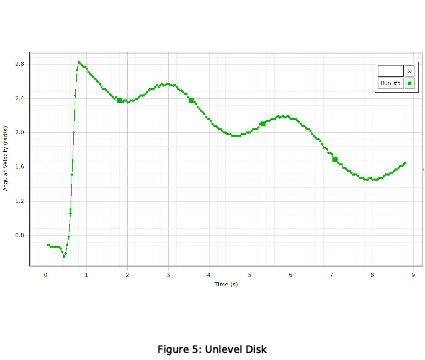
\includegraphics[width=0.9\textwidth, height=0.5\textheight]{/home/vitowu/Documents/e5/JournalSnapshot3.png}
		}
	\end{figure} 
	The level check graph should look like the following figure. There may be some small bumps, but should not be a periodic change caused by the ring speeding up when going downhill and slowing on the uphill portion of its rotation. \par 
	\begin{figure}[H]
		\centering
		\subfigure{}{
			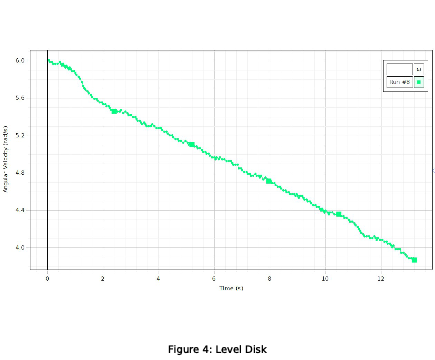
\includegraphics[width=0.9\textwidth, height=0.5\textheight]{/home/vitowu/Documents/e5/JournalSnapshot2.png}
		}
	\end{figure} 
	Repeat leveling the disk until the level check graph looks similar to the accurate figure.\par 
	\subsection{Experiment}
	1. Hold the ring centered on the disk and 2 to 3 mm above it.\par 
	2. Give the disk a clockwise spin (about $20$-$\SI{30}{\radian/\second}$) and start collecting data using 550 Universal Interface. \par 
	3. After about two seconds of data has been taken, drop the ring onto the spinning disk.\par
	4. After another two seconds, stop collecting data and measure the minimum distance between the ring and the edge of the disk.\par
	5. Repeat steps 1-5 two more times.\par 
	~\\
	Use another disk instead of ring and repeat the experiment again. Collect the experimental data respectively.\par 
	
	\section{Experimental Data}
	\subsection{Error Estimation}
	The data we measured include: angular velocity of the system by Rotary Motion Sensor, radius of all objects and mass of all objects.
	\begin{itemize}
		\item Angular Speed: the error is mainly due to the instrument error. According to the manual of Rotary Motion Sensor (PS-2120A), the resolution of the equipment is $0.09\deg$(angular) at 4,000 points per revolution. Therefore, the error we estimated is about $\pm \SI{0.00157}{\radian/\sec}$.
		\item Mass: since the scale has a resolution of 0.01g, the estimated error of mass is $\SI{\pm0.01}{\gram}$.
		\item Radius: the division of the caliper is $\SI{0.05}{\mm}$, so the estimated error of radius is $\SI{\pm0.025}{\mm}$.
		\item x: the estimated error of a common ruler is $\SI{\pm0.05}{\centi\meter}$
	\end{itemize}
	\subsection{Raw Data}
	\begin{figure}[H]
		\centering
		\subfigure{}{
			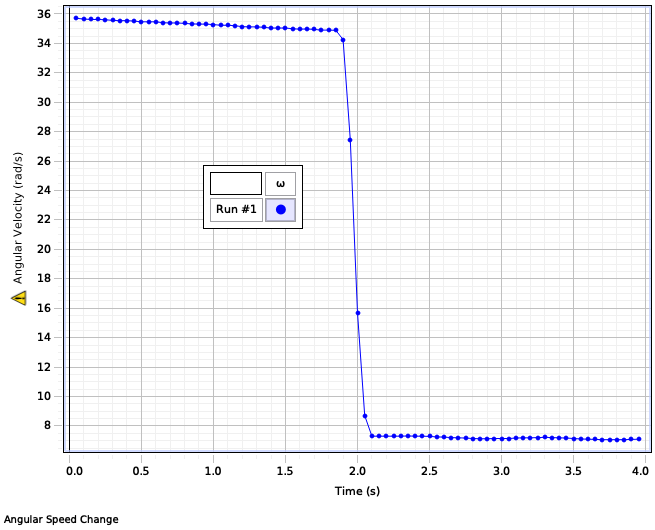
\includegraphics[width=0.45\textwidth]{/home/vitowu/Documents/e5/JournalSnapshot4.png}
			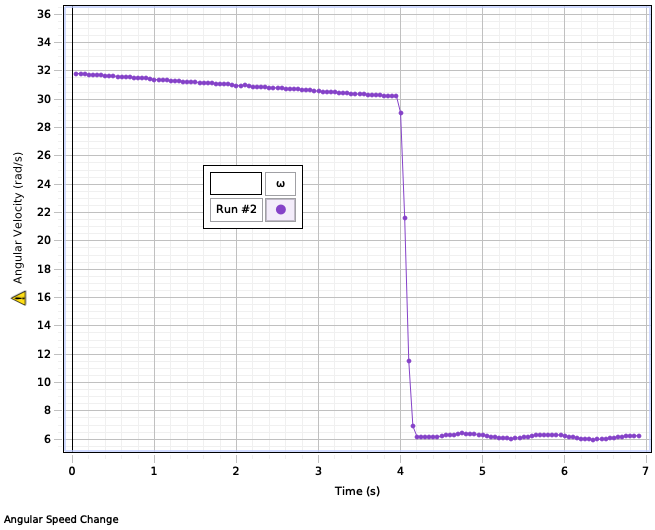
\includegraphics[width=0.45\textwidth]{/home/vitowu/Documents/e5/JournalSnapshot5.png}
			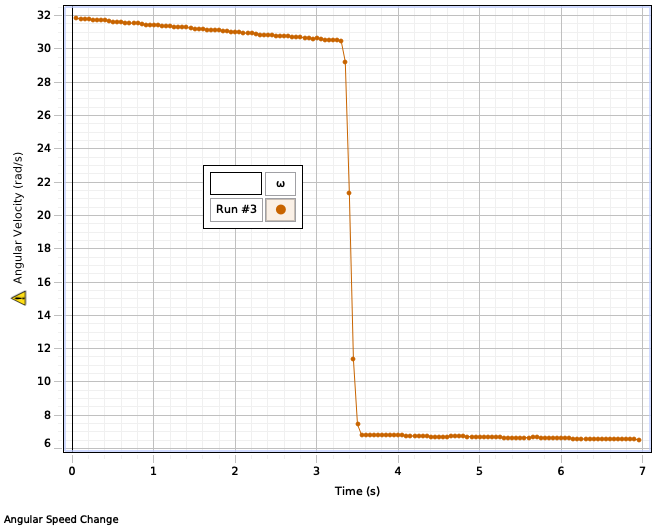
\includegraphics[width=0.45\textwidth]{/home/vitowu/Documents/e5/JournalSnapshot6.png}
			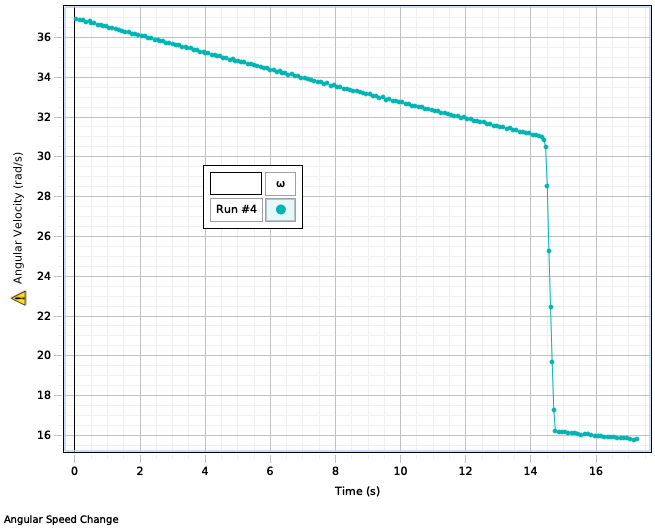
\includegraphics[width=0.45\textwidth]{/home/vitowu/Documents/e5/JournalSnapshot7.png}
		}
	\end{figure}
    Physical Data:
    \begin{table}[H]
    	\centering
    	\makebox[\linewidth]{
    	\begin{tabular}{|c|c|c|c|c|c|c|}
    		\hline
    		\hline
    		Object & $m_{pulley}$($\si{\gram}$) & $r_{pulley}$($\si{\centi\meter}$) & Mass($\si{\gram}$) & $r_{out}$($\si{\centi\meter}$) & $r_{in}$($\si{\centi\meter}$) & x($\si{\centi\meter}$) \\
    		\hline
    		Ring 1& 0.00 & 0.0 & $469.85\pm0.1$ & $3.725\pm0.003$ & $2.6\pm0.003$ & $0.55\pm0.05$ \\
    		\hline
    		Ring 2& 0.00 & 0.0 & $469.85\pm0.1$ & $3.725\pm0.003$ & $2.6\pm0.003$ & $0.56\pm0.05$ \\
    		\hline
    		Ring 3& 0.00 & 0.0 & $469.85\pm0.1$ & $3.725\pm0.003$ & $2.6\pm0.003$ & $0.05\pm0.05$ \\
    		\hline
    		Disk 1& $6.99\pm0.01$ & $2.5\pm0.025$ & $121.94\pm0.1$ & $4.725\pm0.003$ & $0.000$ & $0.00$ \\
    		\hline
    		Disk 2& 0.00 & 0.0 & $120.48\pm0.1$ & $4.725\pm0.003$ & $0.000$ & $0.00$ \\
    		\hline
    	\end{tabular}
    	}
    \end{table}
	Collision Data:
	\begin{table}[H]
		\centering
		\makebox[\linewidth]{
		\begin{tabular}{|c|c|c|}
			\hline
			\hline
			Dropped Object & $\omega_{i}$($\si{\radian/\sec}$) & $\omega_{f}$($\si{\radian/\sec}$) \\
			\hline
			Ring Run 1 & $34.887\pm0.002$ & $7.304\pm0.002$ \\
			\hline
			Ring Run 2 & $30.206\pm0.002$ & $6.189\pm0.002$ \\
			\hline
			Ring Run 3 & $30.473\pm0.002$ & $6.817\pm0.002$ \\
			\hline
			Disk & $30.992\pm0.002$ & $16.211\pm0.002$ \\
			\hline
		\end{tabular}
		}
	\end{table}
	
	\section{Data \& Error Analysis}
	\subsection{Data Calculation}
	According to equation(2) and equation(4), we can calculate the rotational inertia of the disk and the ring, and therefore, by using the equation
	\begin{equation}
		\delta k = \sqrt{\sum_{i=1}^{m}(\frac{\delta f}{\delta p_i})^2(\delta p_i)^2}
	\end{equation}
	we can calculate the error of the computational disk rotational inertia that
	\begin{equation}
		\delta I = \sqrt{(\frac{1}{2}R^2)^2\delta M^2 + (MR)^2\delta R^2}
	\end{equation}
	and the computational ring rotational inertia that
	\begin{equation}
		\delta I = \sqrt{[\frac{1}{2}(R_1^2+R_2^2+2x^2)]^2\delta M^2+(MR_1)^2\delta R_1^2+(MR_2)^2\delta R_2^2+(2Mx)^2\delta x^2}
	\end{equation}\par 
	To calculate the system's total inertia, we can use the equation:
	\begin{equation}
		\delta k = \sqrt{\sum_{i=1}^{m}(c_i\delta p_i)^2}
	\end{equation}
	\begin{table}[H]
		\centering
		\makebox[\linewidth]{
			\begin{tabular}{|c|c|c|c|}
				\hline
				\hline
				 & Object Inertia($\si{\gram\centi\meter^2}$) & Initial Inertia($\si{\gram\centi\meter^2}$) & Final Inertia($\si{\gram\centi\meter^2}$) \\
				\hline
				Ring Run 1 & $4989.954\pm5.492$ & $1383.037\pm1.499$ &  $6372.991\pm6.991$\\
				\hline
				Ring Run 2 & $4995.169\pm5.498$ & $1383.037\pm1.499$ & $6378.206\pm6.997$\\
				\hline
				Ring Run 3 & $4848.999\pm5.339$ & $1383.037\pm1.499$ & $6232.036\pm6.838$\\
				\hline
				Disk & $1344.896\pm1.428$ & $1383.037\pm1.499$ & $2727.933\pm2.927$\\
				\hline
			\end{tabular}
		}
	\end{table}\par
	By equation(1) and equation(2), we can calculate the error of the initial angular momentum and final angular momentum
	\begin{equation}
		\delta L = \sqrt{I^2\delta\omega^2+\omega^2\delta I^2}
	\end{equation}
	Then we can obtain the initial angular momentum and the final angular momentum
	\begin{table}[H]
		\centering
		\makebox[\linewidth]{
			\begin{tabular}{|c|c|c|c|}
				\hline
				\hline
				& Initial L($\si{\gram\centi\meter^2/\sec}$) & Final L($\si{\gram\centi\meter^2/\sec}$) & Difference \\
				\hline
				Ring Run 1 & $48250.012\pm52.341$ & $46548.326\pm52.033$ &  -3.53\% \\
				\hline
				Ring Run 2 & $41776\pm45.331$ & $39474\pm44.447$ & -5.510\% \\
				\hline
				Ring Run 3 & $42145.287\pm45.731$ & $42483.789\pm47.630$ & 0.817\%\\
				\hline
				Disk & $42863.083\pm46.508$ & $44222.522\pm47.642$ & 3.172\% \\
				\hline
			\end{tabular}
		}
	\end{table}\par
	And by equation(5), we can calculate the kinetic energy before and after collision
	\begin{equation}
		\delta KE = \sqrt{(\frac{1}{2}\omega^2)^2\delta I^2 + (2I\omega)^2\delta \omega^2}
	\end{equation}
	\begin{table}[H]
		\centering
		\makebox[\linewidth]{
			\begin{tabular}{|c|c|c|c|}
				\hline
				\hline
				& Initial KE($\si{\gram\centi\meter^2/\sec^2}$) & Final KE($\si{\gram\centi\meter^2/\sec^2}$) & Difference \\
				\hline
				Ring Run 1 & $841649.081\pm924.714$ & $169994.488\pm236.934$ &  -79.802\% \\
				\hline
				Ring Run 2 & $630943.164\pm696.313$ & $122154.512\pm182.541$ & -80.639\% \\
				\hline
				Ring Run 3 & $642146.658\pm708.458$ & $144805.996\pm207.461$ & -77.450\%\\
				\hline
				Disk & $664206.330\pm732.371$ & $358445.951\pm408.902$ & -46.034\% \\
				\hline
			\end{tabular}
		}
	\end{table}\par
	\subsection{Analysis of Data}
	As the above data shows that the differences of angular momentum before and after collision are within 6\%, considering the possible error, it is reasonable and acceptable to conclude that the experimental results satisfy the theoretical expectations. \par
	In addition, the last result table of KE shows that the kinetic energy are not conserved in experiment, and with a significant energy loss over 45\% after collision. As what we suggested in pre-experiment questions, the collision is an inelastic collision.
	
	\section{Conclusion}
	During the experiment, we used a non-rotating ring, a non-rotating disk and a rotating disk and dropped the non-rotating ring \& non-rotating disk onto the rotating disk respectively. We performed the dropping for 4 times and collected the experimental data. Last, we gave a sufficient error analysis on each data we collected and each result we calculated from the data. Compared with the theoretical equations on Law of Conservation of Angular Momentum, we can conclude that
	\begin{itemize}
		\item The experimental result supports the Law of Conservation of Angular Momentum. In the experiment, we found that the system angular momentum before and after collisions are approximately the same (within 6\% difference). Considering possible error caused by measurements and instruments, we strongly believed that, our experimental result satisfies the theory and supports the theory.
		\item The Kinetic Energy was not conserved in the collision. In the experiment, we found that the kinetic energy of the system presented a significant loss after the collision, that the dropping of ring caused an energy loss about 80\% and the dropping of disk caused an energy loss about 46.034\%.
	\end{itemize}
	
	\section{Extension Questions}
	\subsection{What affect on the value you calculate for the final angular momentum.}
	\subsubsection{If the Rotary Motion Sensor has a small rotational inertia.}
	If the Rotary Motion Sensor has a small rotational inertia, the final angular momentum would be smaller, since that we omitted the small rotational inertia on pulley in calculation, and however, the total angular momentum of the system was conversed, it means that the final angular momentum would be smaller.
	\subsubsection{If the frictional drag on the bearings during the collision cannot be ignored}
	If the frictional drag on the bearings during the collision cannot be ignored, the final angular momentum would be smaller, since the frictional drag would result in a torque that decrease the angular speed of the disk. Thus, the final angular speed would be less, which means the final angular momentum would also be less. 
	\subsection{Typically, you should see a loss of angular moment for the ring of 5\%-15\%. If you did the disk drop, it should have shown a drop of a few percent.}
	\subsubsection{Why should the disk drop work better?}
	We suggest that the reason may be relative to that the ring was not being dropped in the center of the disk perfectly and caused the disk tended to incline. And therefore there was a friction between the disk and the supporting rod, which might caused a torque on the disk. Like what we suggested above, this torque will decrease the angular momentum of the entire system.
	\subsubsection{Despite the fact that it works better, the disk drop does not provide convincing evidence for the general rule. Why not?}
	Since that the mass and the radius of the two disks are approximately the same, the final angular speed will also be approximately the same. It is a special case of the conservation of angular momentum, and if we want the experiment to be more general, we need to use objects with different mass and different radius.
	\subsection{How can angular momentum be conserved, but energy not be conserved?}
	During the experiment, there was no outside torque on the system, and therefore the angular momentum was conserved. During the collision, however, some of the kinetic energy may became thermal energy due to the friction between rotating disk and the dropping object.
\end{document}